% -----------------------------------------------
% Template for SMC 2020
% adapted from previous SMC paper templates
% -----------------------------------------------

\documentclass{article}
\usepackage{smc2020}
\usepackage{times}
\usepackage{ifpdf}
\usepackage[english]{babel}
\usepackage{cite}

%%%%%%%%%%%%%%%%%%%%%%%% Some useful packages %%%%%%%%%%%%%%%%%%%%%%%%%%%%%%%
%%%%%%%%%%%%%%%%%%%%%%%% See related documentation %%%%%%%%%%%%%%%%%%%%%%%%%%
%\usepackage{amsmath} % popular packages from Am. Math. Soc. Please use the
%\usepackage{amssymb} % related math environments (split, subequation, cases,
%\usepackage{amsfonts}% multline, etc.)
%\usepackage{bm}      % Bold Math package, defines the command \bf{}
%\usepackage{paralist}% extended list environments
%%subfig.sty is the modern replacement for subfigure.sty. However, subfig.sty
%%requires and automatically loads caption.sty which overrides class handling
%%of captions. To prevent this problem, preload caption.sty with caption=false
%\usepackage[caption=false]{caption}
%\usepackage[font=footnotesize]{subfig}


%user defined variables
\def\papertitle{SEAM PROJECT - SUSTAINED STEREOPHONY}
\def\firstauthor{Giuseppe Silvi}
\def\secondauthor{Davide Tedesco}
\def\thirdauthor{Third author}

% adds the automatic
% Saves a lot of output space in PDF... after conversion with the distiller
% Delete if you cannot get PS fonts working on your system.

% pdf-tex settings: detect automatically if run by latex or pdflatex
\newif\ifpdf
\ifx\pdfoutput\relax
\else
   \ifcase\pdfoutput
      \pdffalse
   \else
      \pdftrue
\fi

\ifpdf % compiling with pdflatex
  \usepackage[pdftex,
    pdftitle={\papertitle},
    pdfauthor={\firstauthor, \secondauthor, \thirdauthor},
    bookmarksnumbered, % use section numbers with bookmarks
    pdfstartview=XYZ % start with zoom=100% instead of full screen;
                     % especially useful if working with a big screen :-)
   ]{hyperref}
  %\pdfcompresslevel=9

  \usepackage[pdftex]{graphicx}
  % declare the path(s) where your graphic files are and their extensions so
  %you won't have to specify these with every instance of \includegraphics
  \graphicspath{{img/}}
  \DeclareGraphicsExtensions{.pdf,.jpeg,.png}

  \usepackage[figure,table]{hypcap}

\else % compiling with latex
  \usepackage[dvips,
    bookmarksnumbered, % use section numbers with bookmarks
    pdfstartview=XYZ % start with zoom=100% instead of full screen
  ]{hyperref}  % hyperrefs are active in the pdf file after conversion

  \usepackage[dvips]{epsfig,graphicx}
  % declare the path(s) where your graphic files are and their extensions so
  %you won't have to specify these with every instance of \includegraphics
  \graphicspath{{./figures/}}
  \DeclareGraphicsExtensions{.eps}

  \usepackage[figure,table]{hypcap}
\fi

%setup the hyperref package - make the links black without a surrounding frame
\hypersetup{
    colorlinks,%
    citecolor=black,%
    filecolor=black,%
    linkcolor=black,%
    urlcolor=black
}

\usepackage{color}
\usepackage{listings}
\definecolor{mygrey}{rgb}{0.96,0.96,0.96}
\lstset{
  tabsize=4,
  basicstyle=\ttfamily,
  backgroundcolor=\color{mygrey},
  captionpos=b,
  breaklines=true
}


% Title.
% ------
\title{\papertitle}

% Authors
% Please note that submissions are NOT anonymous, therefore
% authors' names have to be VISIBLE in your manuscript.
%
% Single address
% To use with only one author or several with the same address
% ---------------
%\oneauthor
%   {\firstauthor} {Affiliation1 \\ %
%     {\tt \href{mailto:author1@smcnetwork.org}{author1@smcnetwork.org}}}

%Two addresses
%--------------
 \twoauthors
   {\firstauthor} {Affiliation1 \\ %
     {\tt \href{mailto:author1@smcnetwork.org}{author1@smcnetwork.org}}}
   {\secondauthor} {Affiliation2 \\ %
     {\tt \href{mailto:author2@smcnetwork.org}{author2@smcnetwork.org}}}

% Three addresses
% --------------
% \threeauthors
%   {\firstauthor} {Affiliation1 \\ %
%     {\tt \href{mailto:author1@smcnetwork.org}{author1@smcnetwork.org}}}
%   {\secondauthor} {Affiliation2 \\ %
%     {\tt \href{mailto:author2@smcnetwork.org}{author2@smcnetwork.org}}}
%   {\thirdauthor} { Affiliation3 \\ %
%     {\tt \href{mailto:author3@smcnetwork.org}{author3@smcnetwork.org}}}


%%%%%%%%%%%%%%%%%%%%%%%%%%%%%%%%%%%%%%%%%%%%%%%%%%%%%%% THE DOCUMENT STARTS HERE
\begin{document}
%
\capstartfalse
\maketitle
\capstarttrue
%
\begin{abstract}
\input{abstract.txt}
\end{abstract}
%

\section{Introduction}
\label{sec:introduction}

\emph{Sustained Electro-Acoustic Music} is a project inspired by Alvise Vidolin
and Nicola Bernardini's article \cite{bevi05} on \emph{live electroacoustic
music sustainability}.

The main ambition of this project is to grow the interpretation and the
electroacoustic musical practice with the consciousness of the electronic
and informatics problems that had made arduous to approach this music and
prevented the growth of interpretative thinking. It is possible, with a
community structure, to determine, build and stratify interpretation of musical
core, the repertoire, concealing the environment-related technological issues.
They are instruments, not the music itself, after all.

These are the SEAM organisation coordinates:
\begin{itemize}
\item \url{http://s-e-a-m.github.io}
\item \url{http://seam-world.slack.com}
\end{itemize}

\section{PROBLEMS}
\label{sec:problems}

Why a project about sustained electroacoustic music must focus on stereophony
issues? The literature and the repertoire survive thanks to the community
activities. Most of those activities require education, strong education about
musical matters. The education, even music education, is layered, from roots
to top floor of music knowledge. To look inside the twenty-third floor, you
have acquired the bottom levels of knowledge, from the roots.

Especially the roots, the elementary concepts, the etymology of the basic lexis,
is the most fragile and most violated place of knowledge, a place where
stereophony, one of the keywords of the sound realm, just before to lose its
meaning still losing its necessity.

During the lessons in Rome Conservatory in which \emph{SEAM} was born and its
related problems were shared with classes to sensitize students to community
work, the core software used to explode issues was \emph{Faust}\footnote{
\url{https://faust.grame.fr}}. This wasn't a restriction, it was a preference.
Text-based DSP offers the deepest learning experience and great expressivity
and readability. \emph{Faust} code could be written to educate a musician at
the same time with computation versatility and efficiency. The \emph{Faust
libraries} concept is useful to focus on write once, and read forever, code.
We think \emph{Faust} itself represents a rather concept of electroacoustic sustainability. Thinking, for example, at the \emph{filters.lib} and at the
names that contributed the enrichment of speculation around each object, make
us wish to a musical interest capable to do community more than with the
adoption of other software.

Instruments carved by musical ideas on readable text (code) becomes a
sub-literature in which each brick maintain the power of the source code, the
clarity of an equation, the efficiency of the continuous development, the
reusability of a word in different contexts.

\section{ROOTS}
\label{sec:roots}

Blumlein

\section{Mid-Side Panner}
\label{sec:mspanner}

%--------------------------------------------
%----------------larghezza massima del codice
\begin{lstlisting}
import("stdfaust.lib");
import("../faust-libraries/seam.lib");
\end{lstlisting}

%\section{Floats and equations}
%
%\subsection{Equations}
%Equations should be placed on separated lines and numbered. The number should be on the right side, in parentheses.
%\begin{equation}
%r=\sqrt[13]{3}
%\label{eq:BP}
%\end{equation}
%Always refer to equations like this: ``Equation (\ref{eq:BP}) is of particular interest because...''
%
%\subsection{Figures, Tables and Captions}
%\begin{table}[t]
% \begin{center}
% \begin{tabular}{|l|l|}
%  \hline
%  String value & Numeric value \\
%  \hline
%  Moin! SMC & 2020 \\
%  \hline
% \end{tabular}
%\end{center}
% \caption{Table captions should be placed below the table,  like this.}
% \label{tab:example}
%\end{table}
%
%All artwork must be centered, neat, clean and legible. Figures should be centered, neat, clean
%and completely legible. All lines should be thick and dark enough for purposes of reproduction. Artwork should not be hand-drawn. The proceedings will be distributed in electronic form only, therefore color figures are allowed. However, you may want to check that your figures are understandable even if they are printed in black-and-white.
%
%
%Numbers and captions of figures and tables always appear below the figure/table.
%Leave 1 line space between the figure or table and the caption.
%Figure and tables are numbered consecutively.
%Captions should be Times 10pt. Place tables/figures in the text as close to the reference as possible,
%and preferably at the top of the page.
%
%Always refer to tables and figures in the main text, for example: ``see Fig. \ref{fig:example} and \tabref{tab:example}''.
%Figures and tables may extend across both columns to a maximum width of 17.2cm.
%
%Vectorial figures are preferred, e.g., eps. When using \texttt{Matlab}, export using either (encapsulated) Postscript or PDF format. In order to optimize readability, the font size of text within a figure should be no smaller than
%that of footnotes (8~pt font-size). If you use bitmap figures, make sure that the resolution is high enough for print quality.

\begin{figure}[t]
\centering
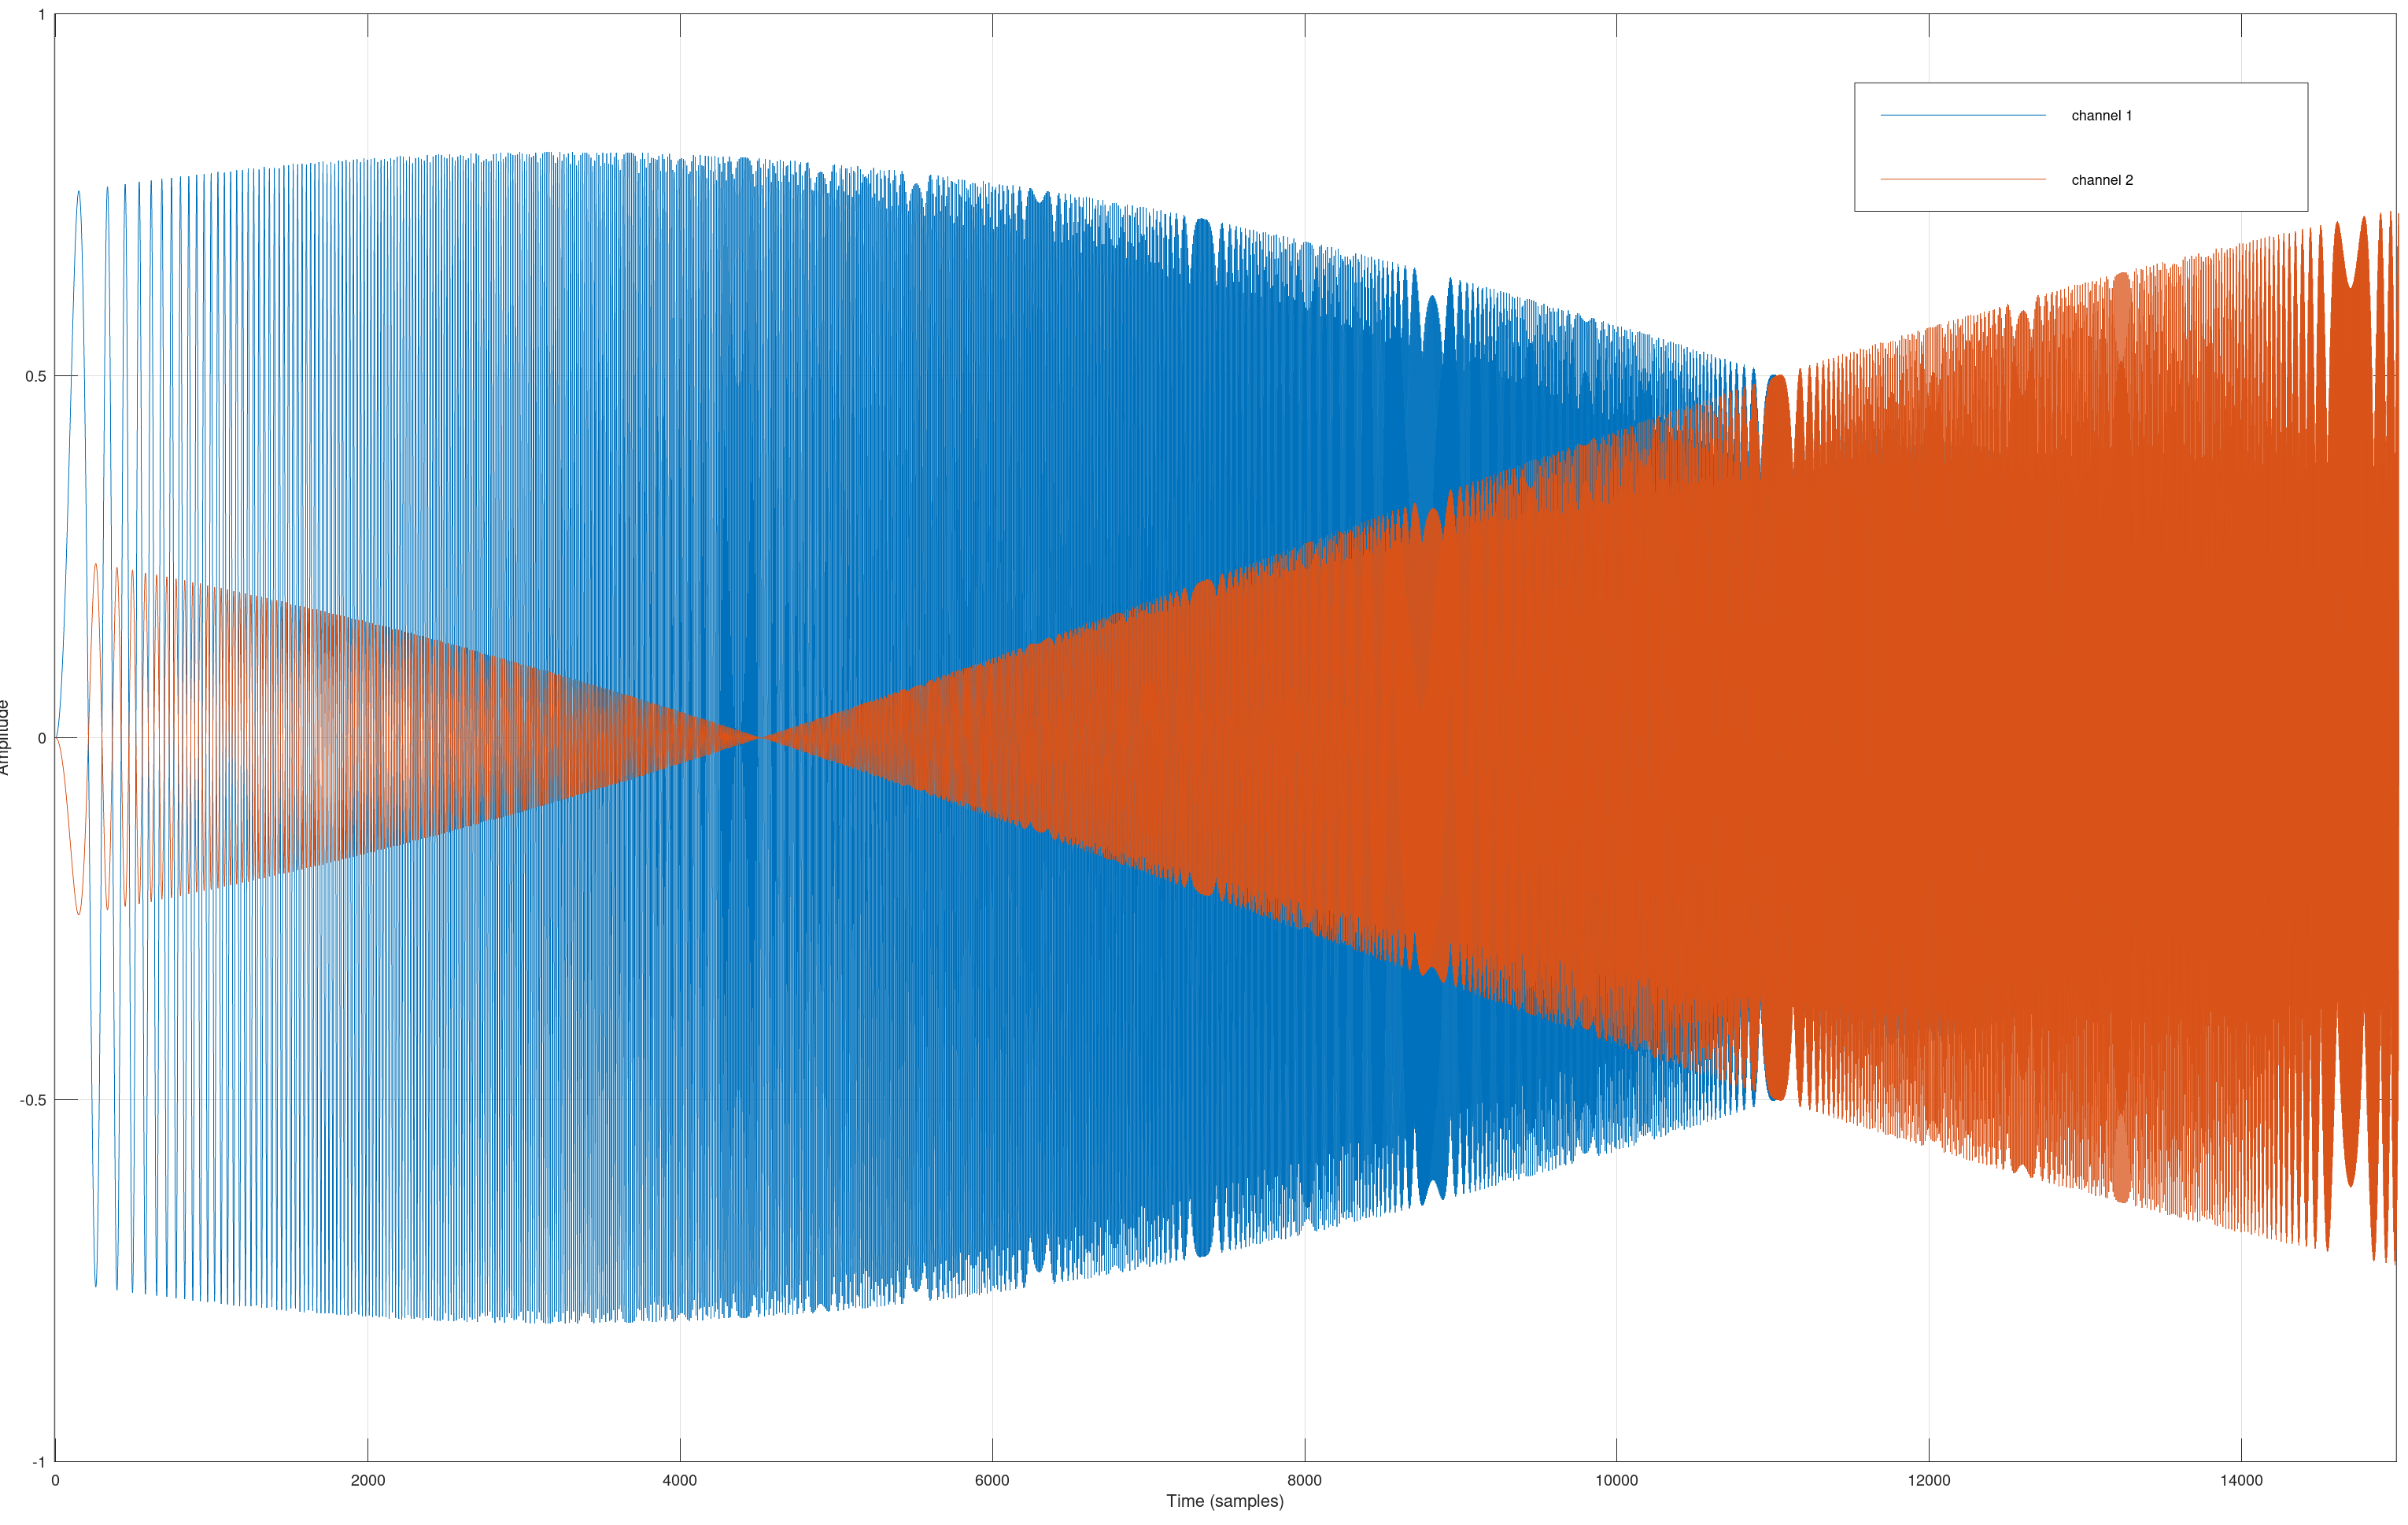
\includegraphics[width=1\columnwidth]{MS2LR-90deg}
\caption{Figure captions should be placed below the figure,
exactly like this.\label{fig:example}}
\end{figure}

\begin{figure}[t]
\centering
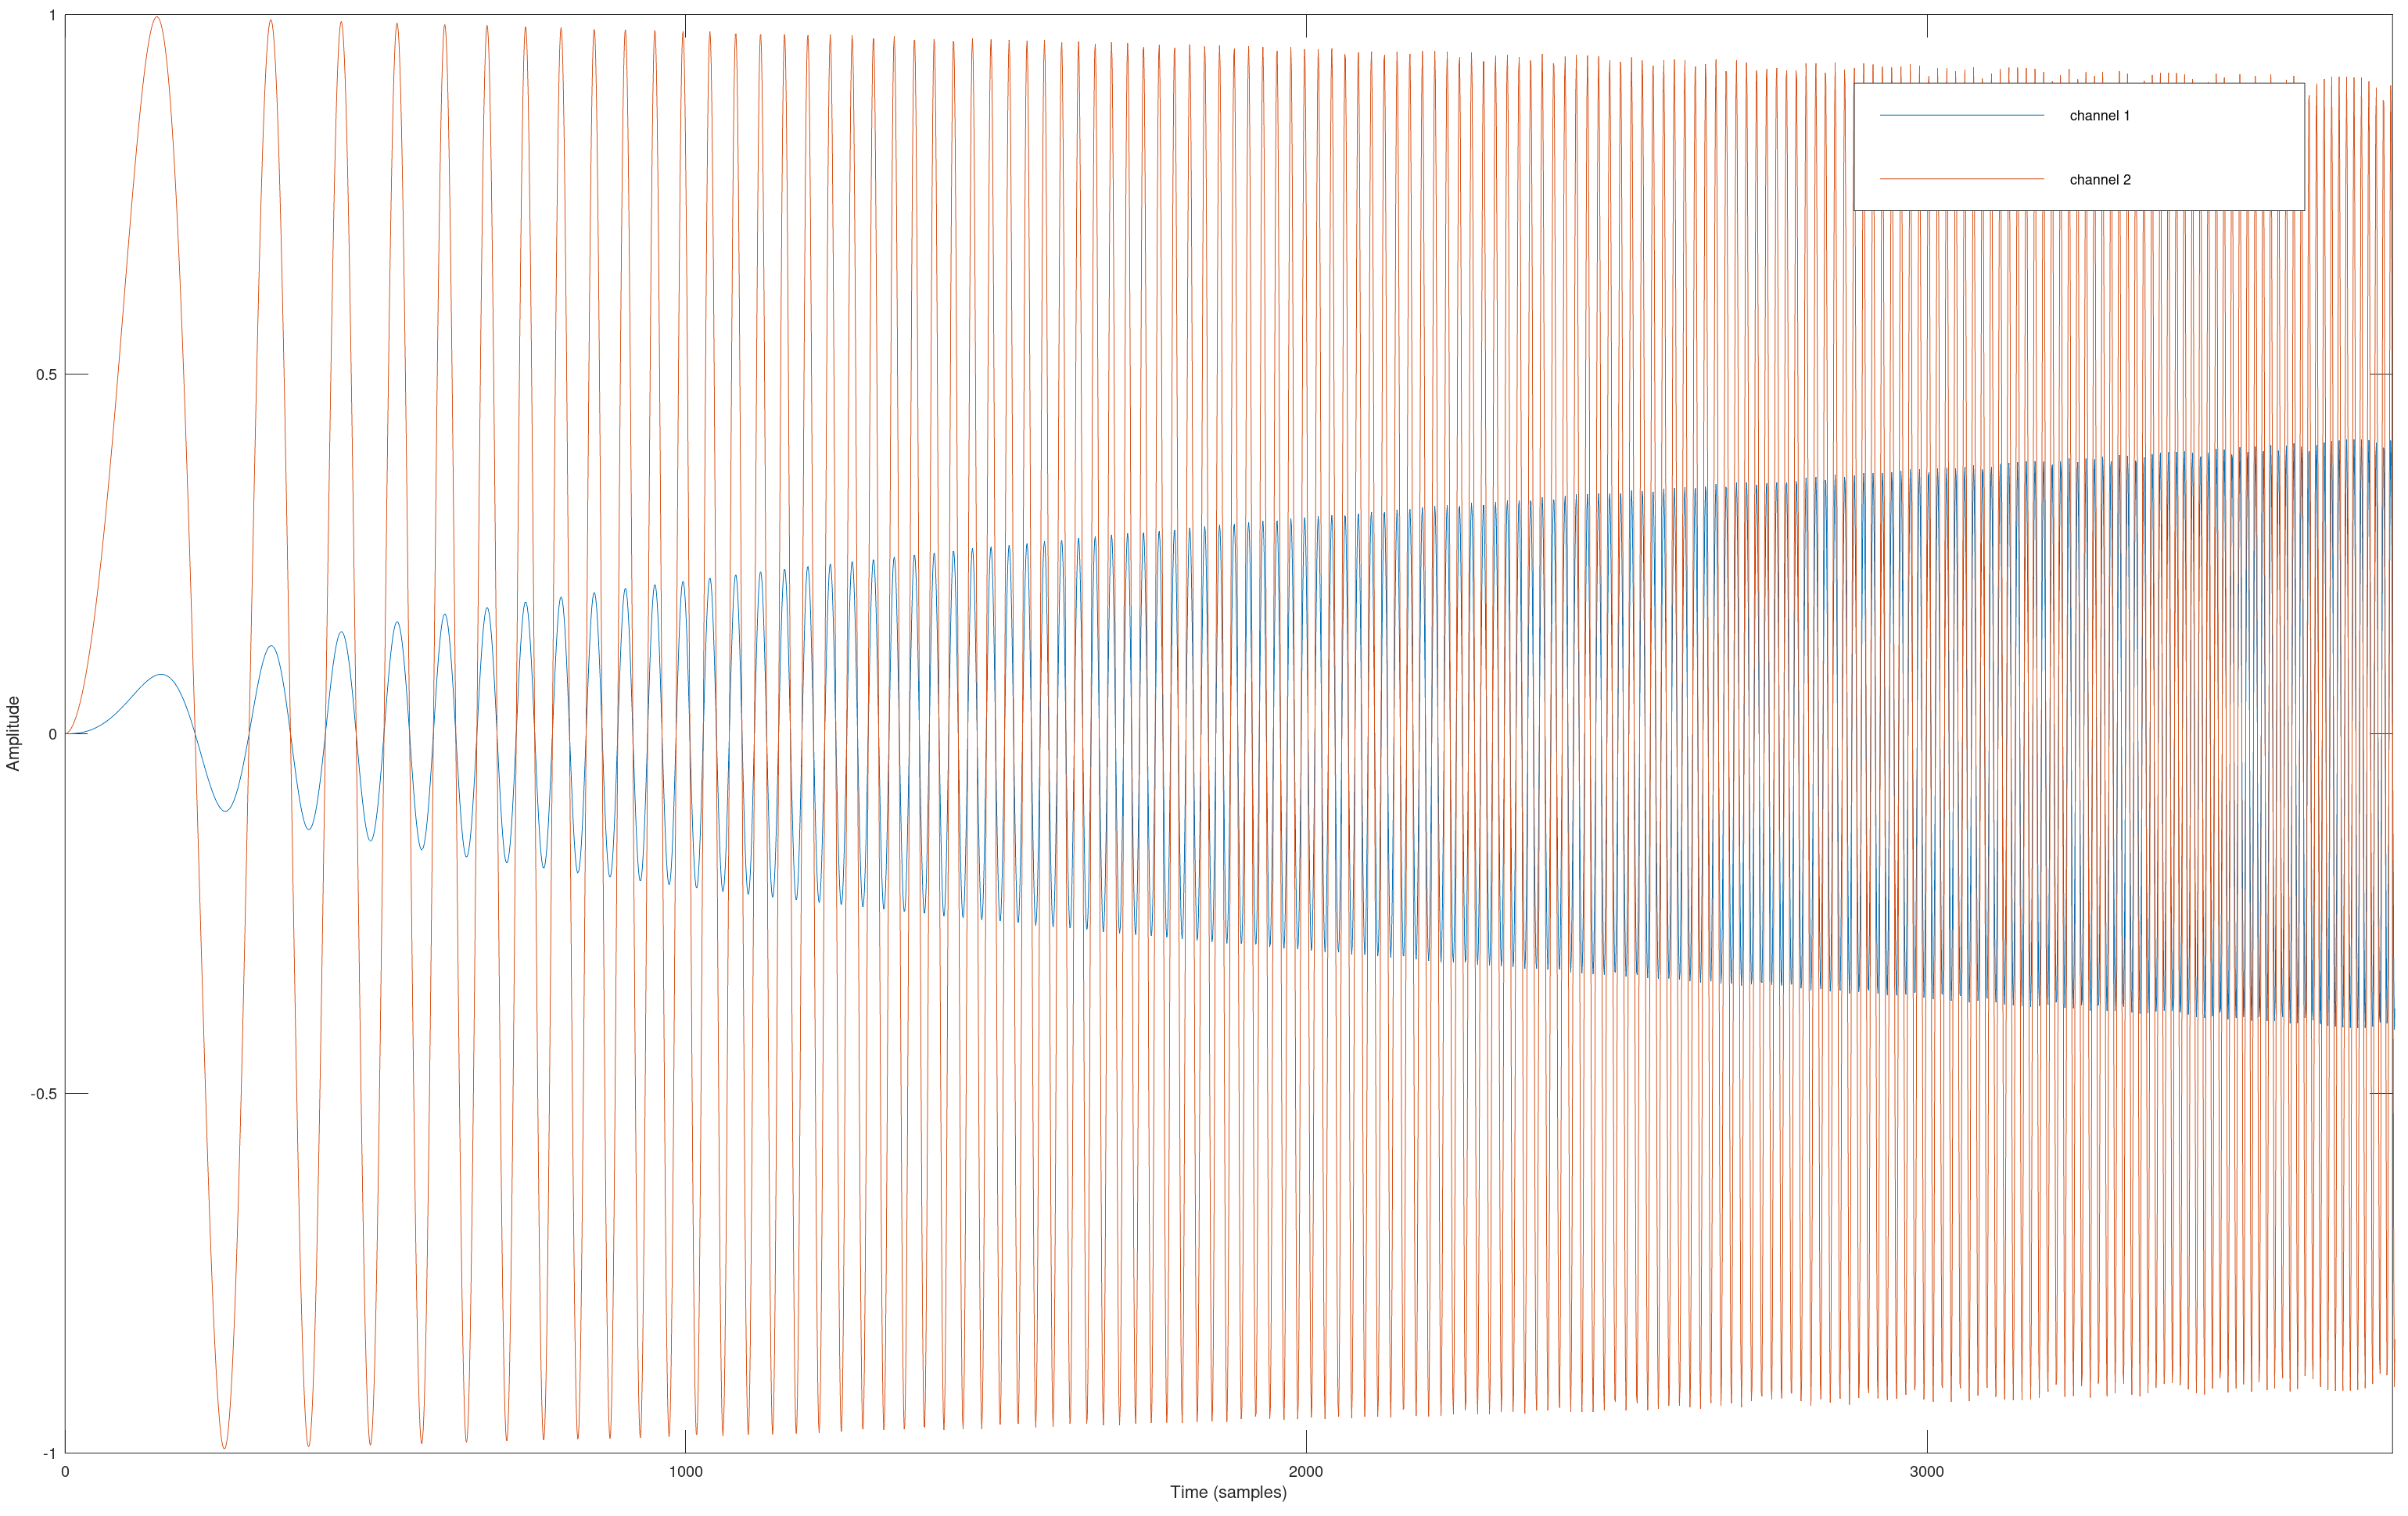
\includegraphics[width=1\columnwidth]{SQRT-LR}
\caption{Figure captions should be placed below the figure,
exactly like this.\label{fig:example}}
\end{figure}

\begin{figure}[t]
\centering
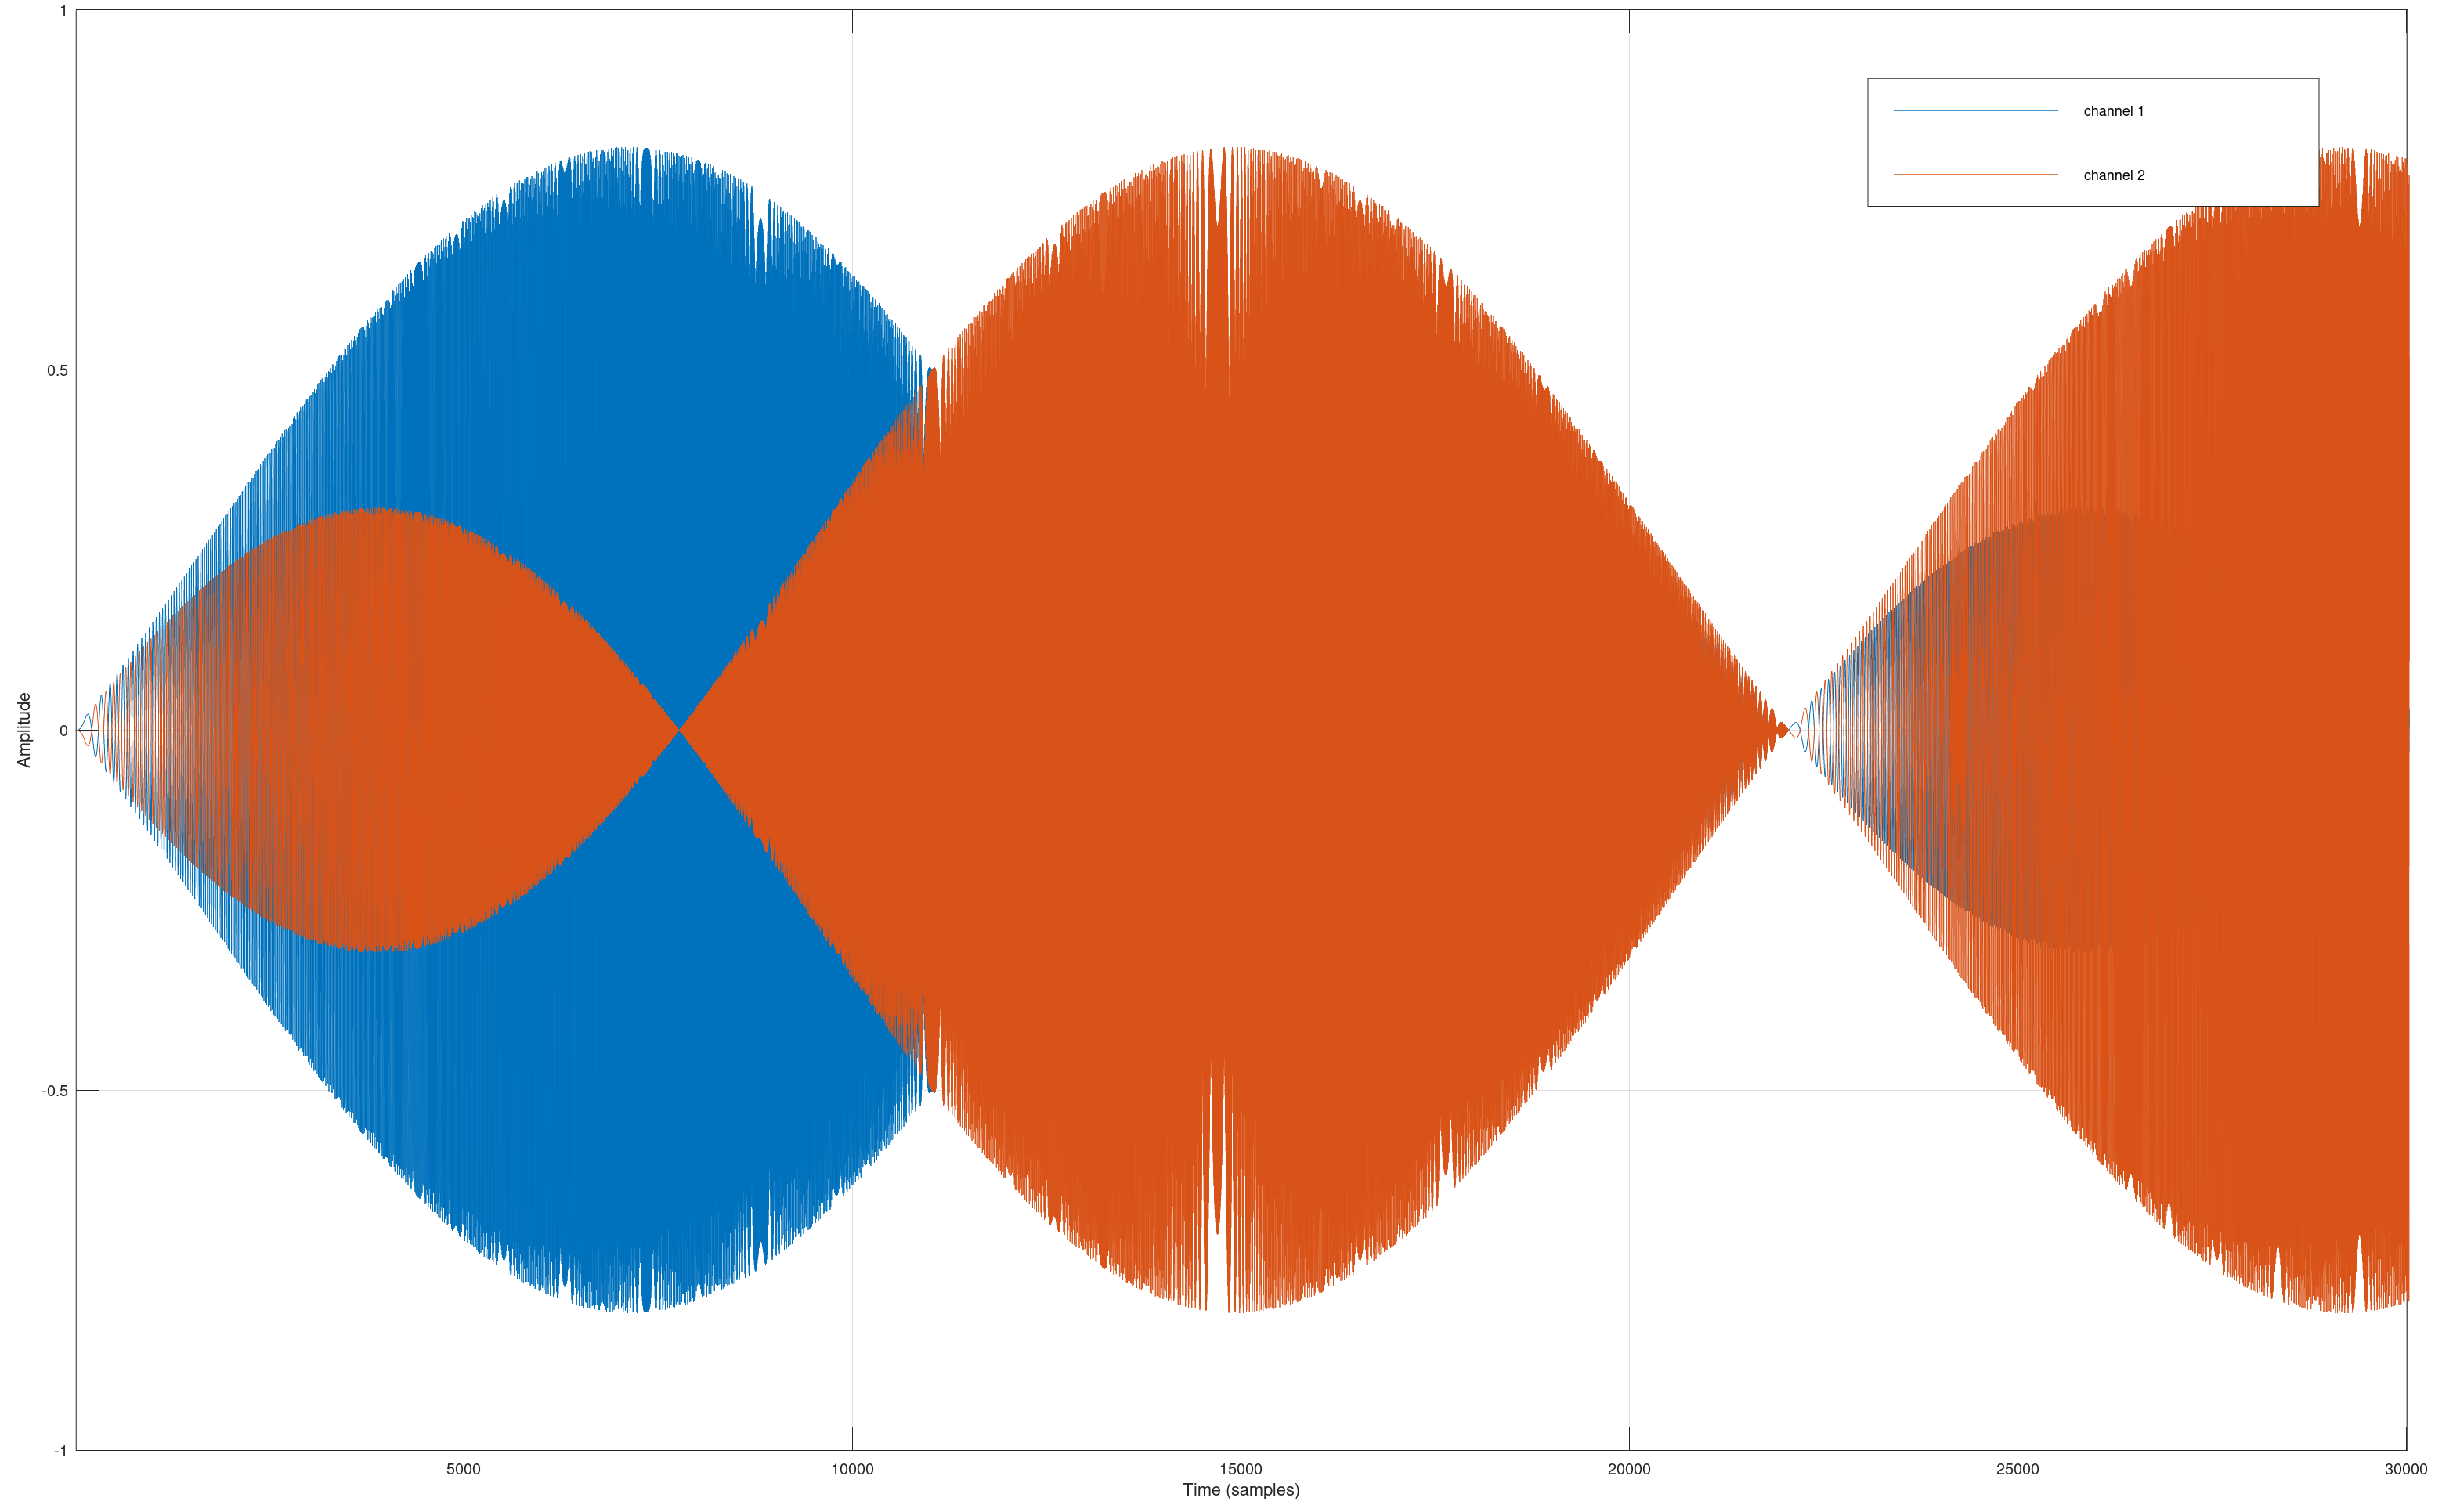
\includegraphics[width=1\columnwidth]{MS2LR-180deg-1}
\caption{Figure captions should be placed below the figure,
exactly like this.\label{fig:example}}
\end{figure}

\begin{figure}[t]
\centering
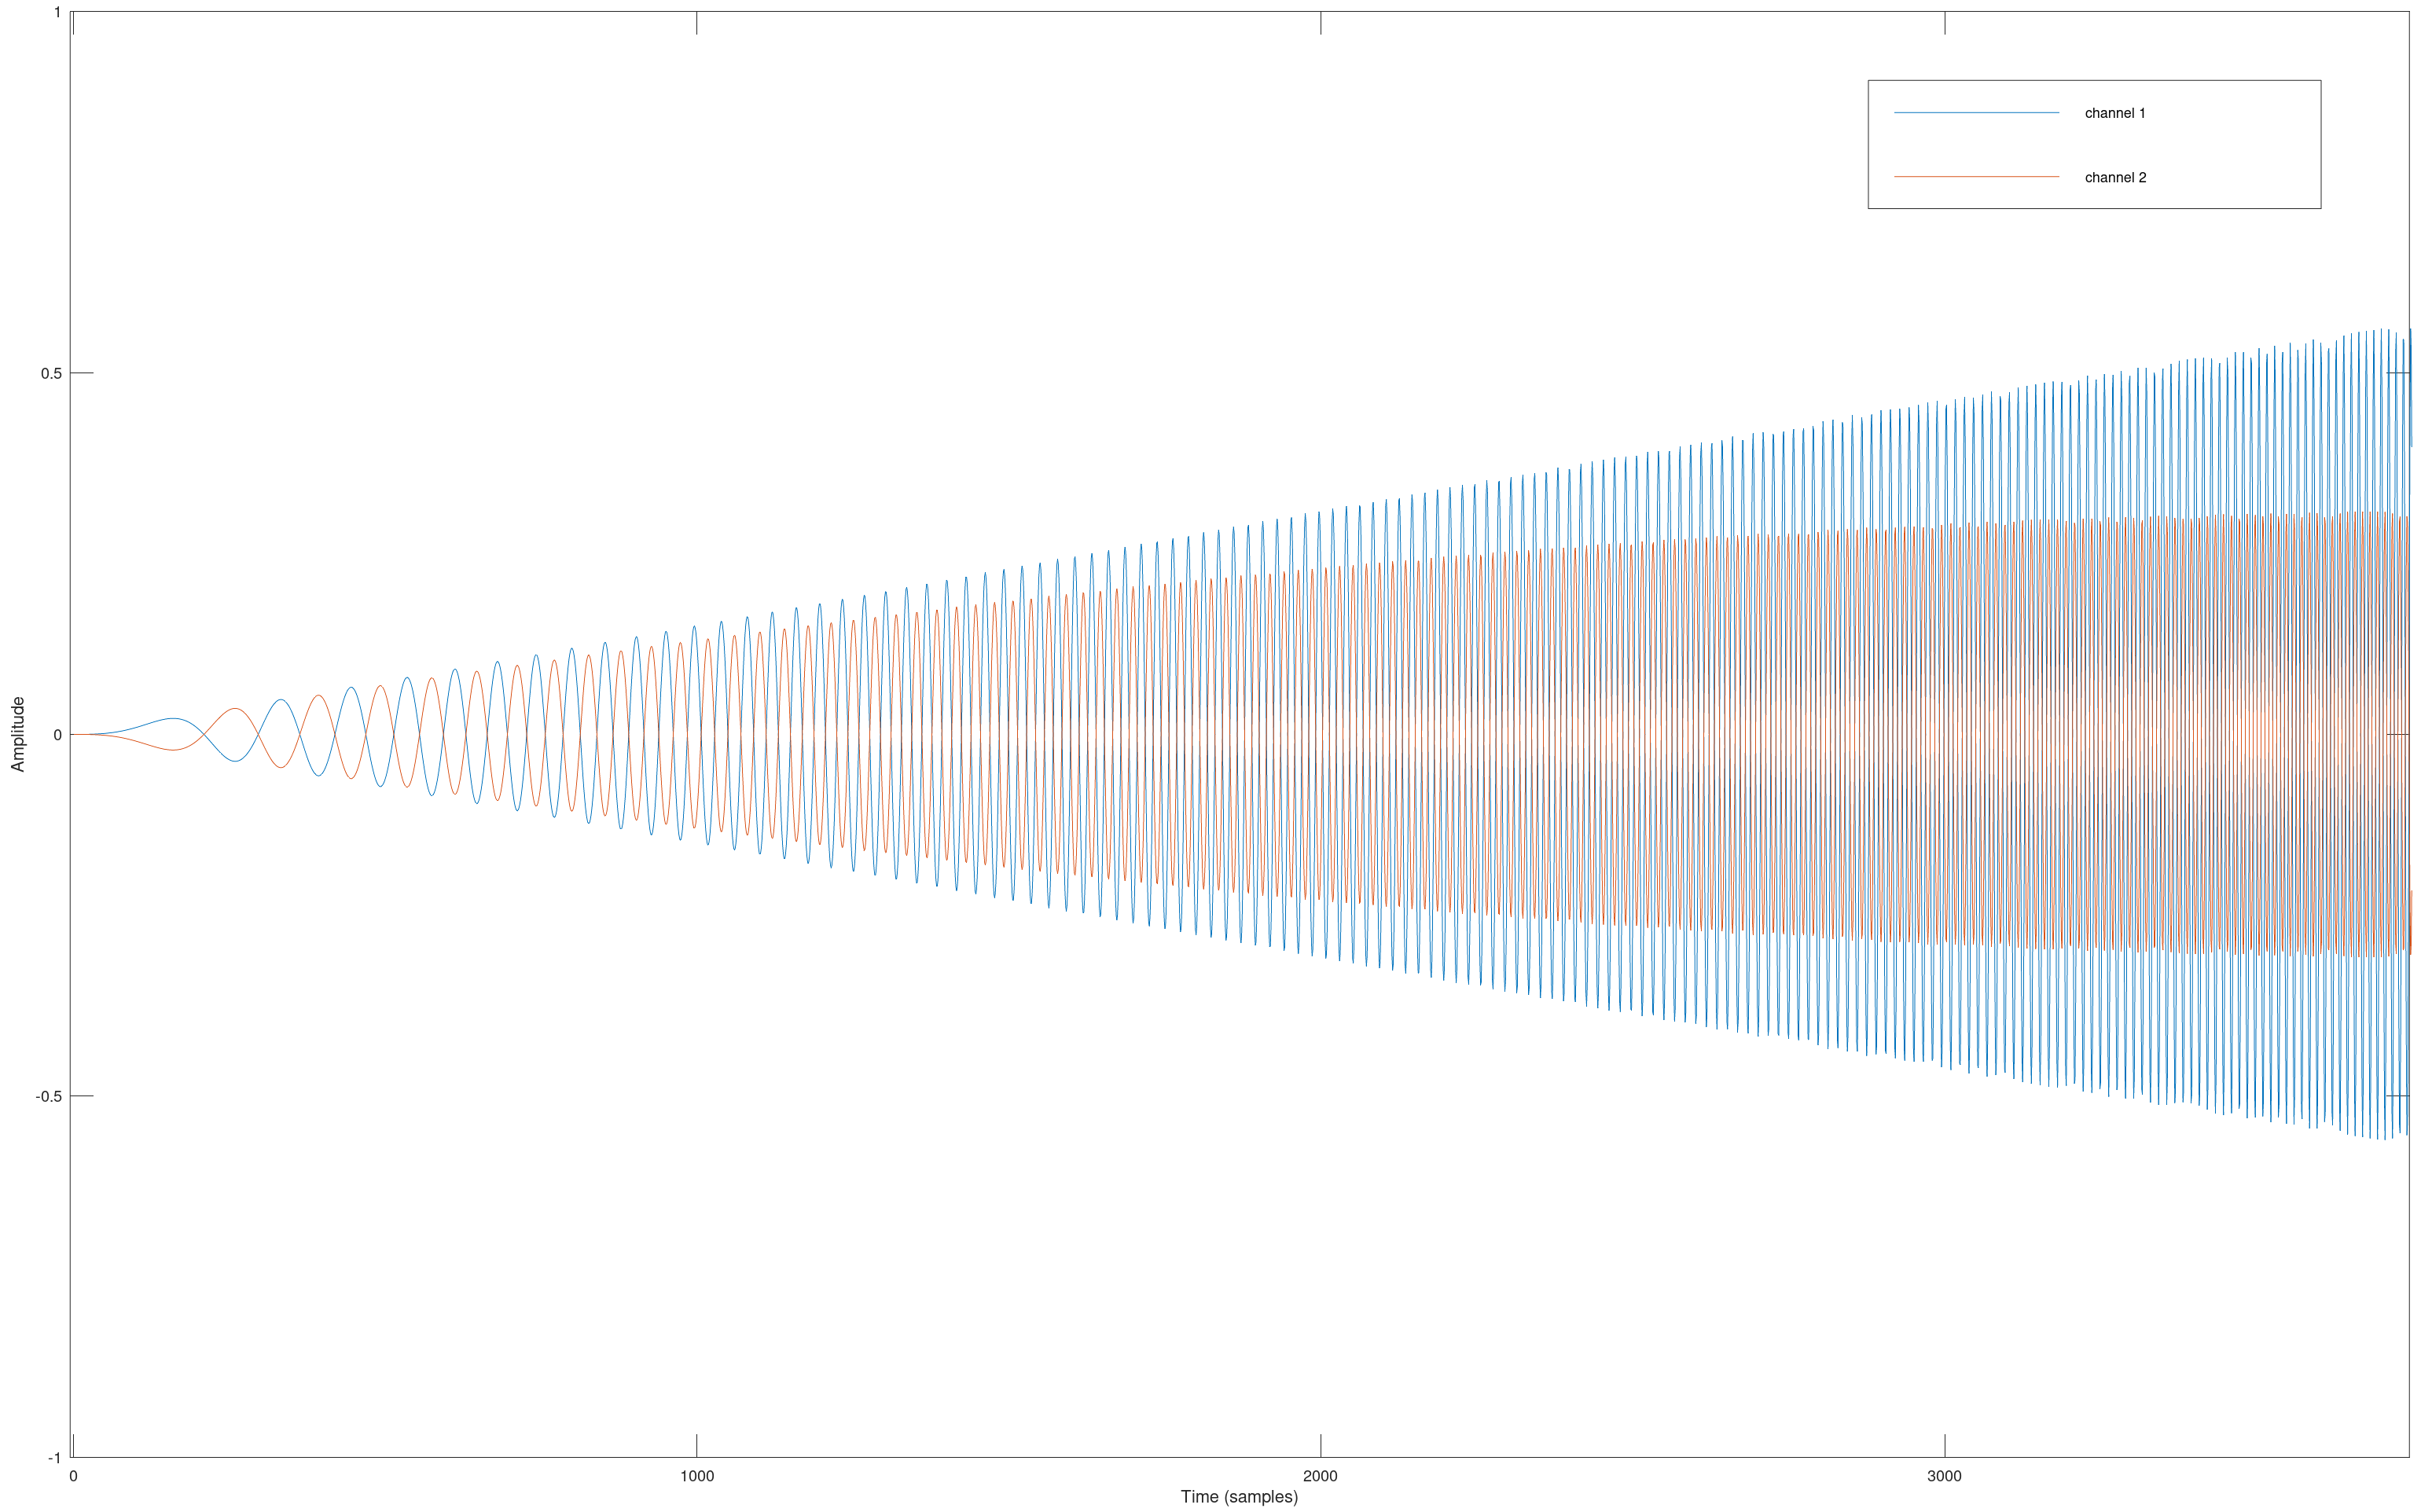
\includegraphics[width=1\columnwidth]{MS2LR-180deg-2}
\caption{Figure captions should be placed below the figure,
exactly like this.\label{fig:example}}
\end{figure}

\begin{figure}[t]
\centering
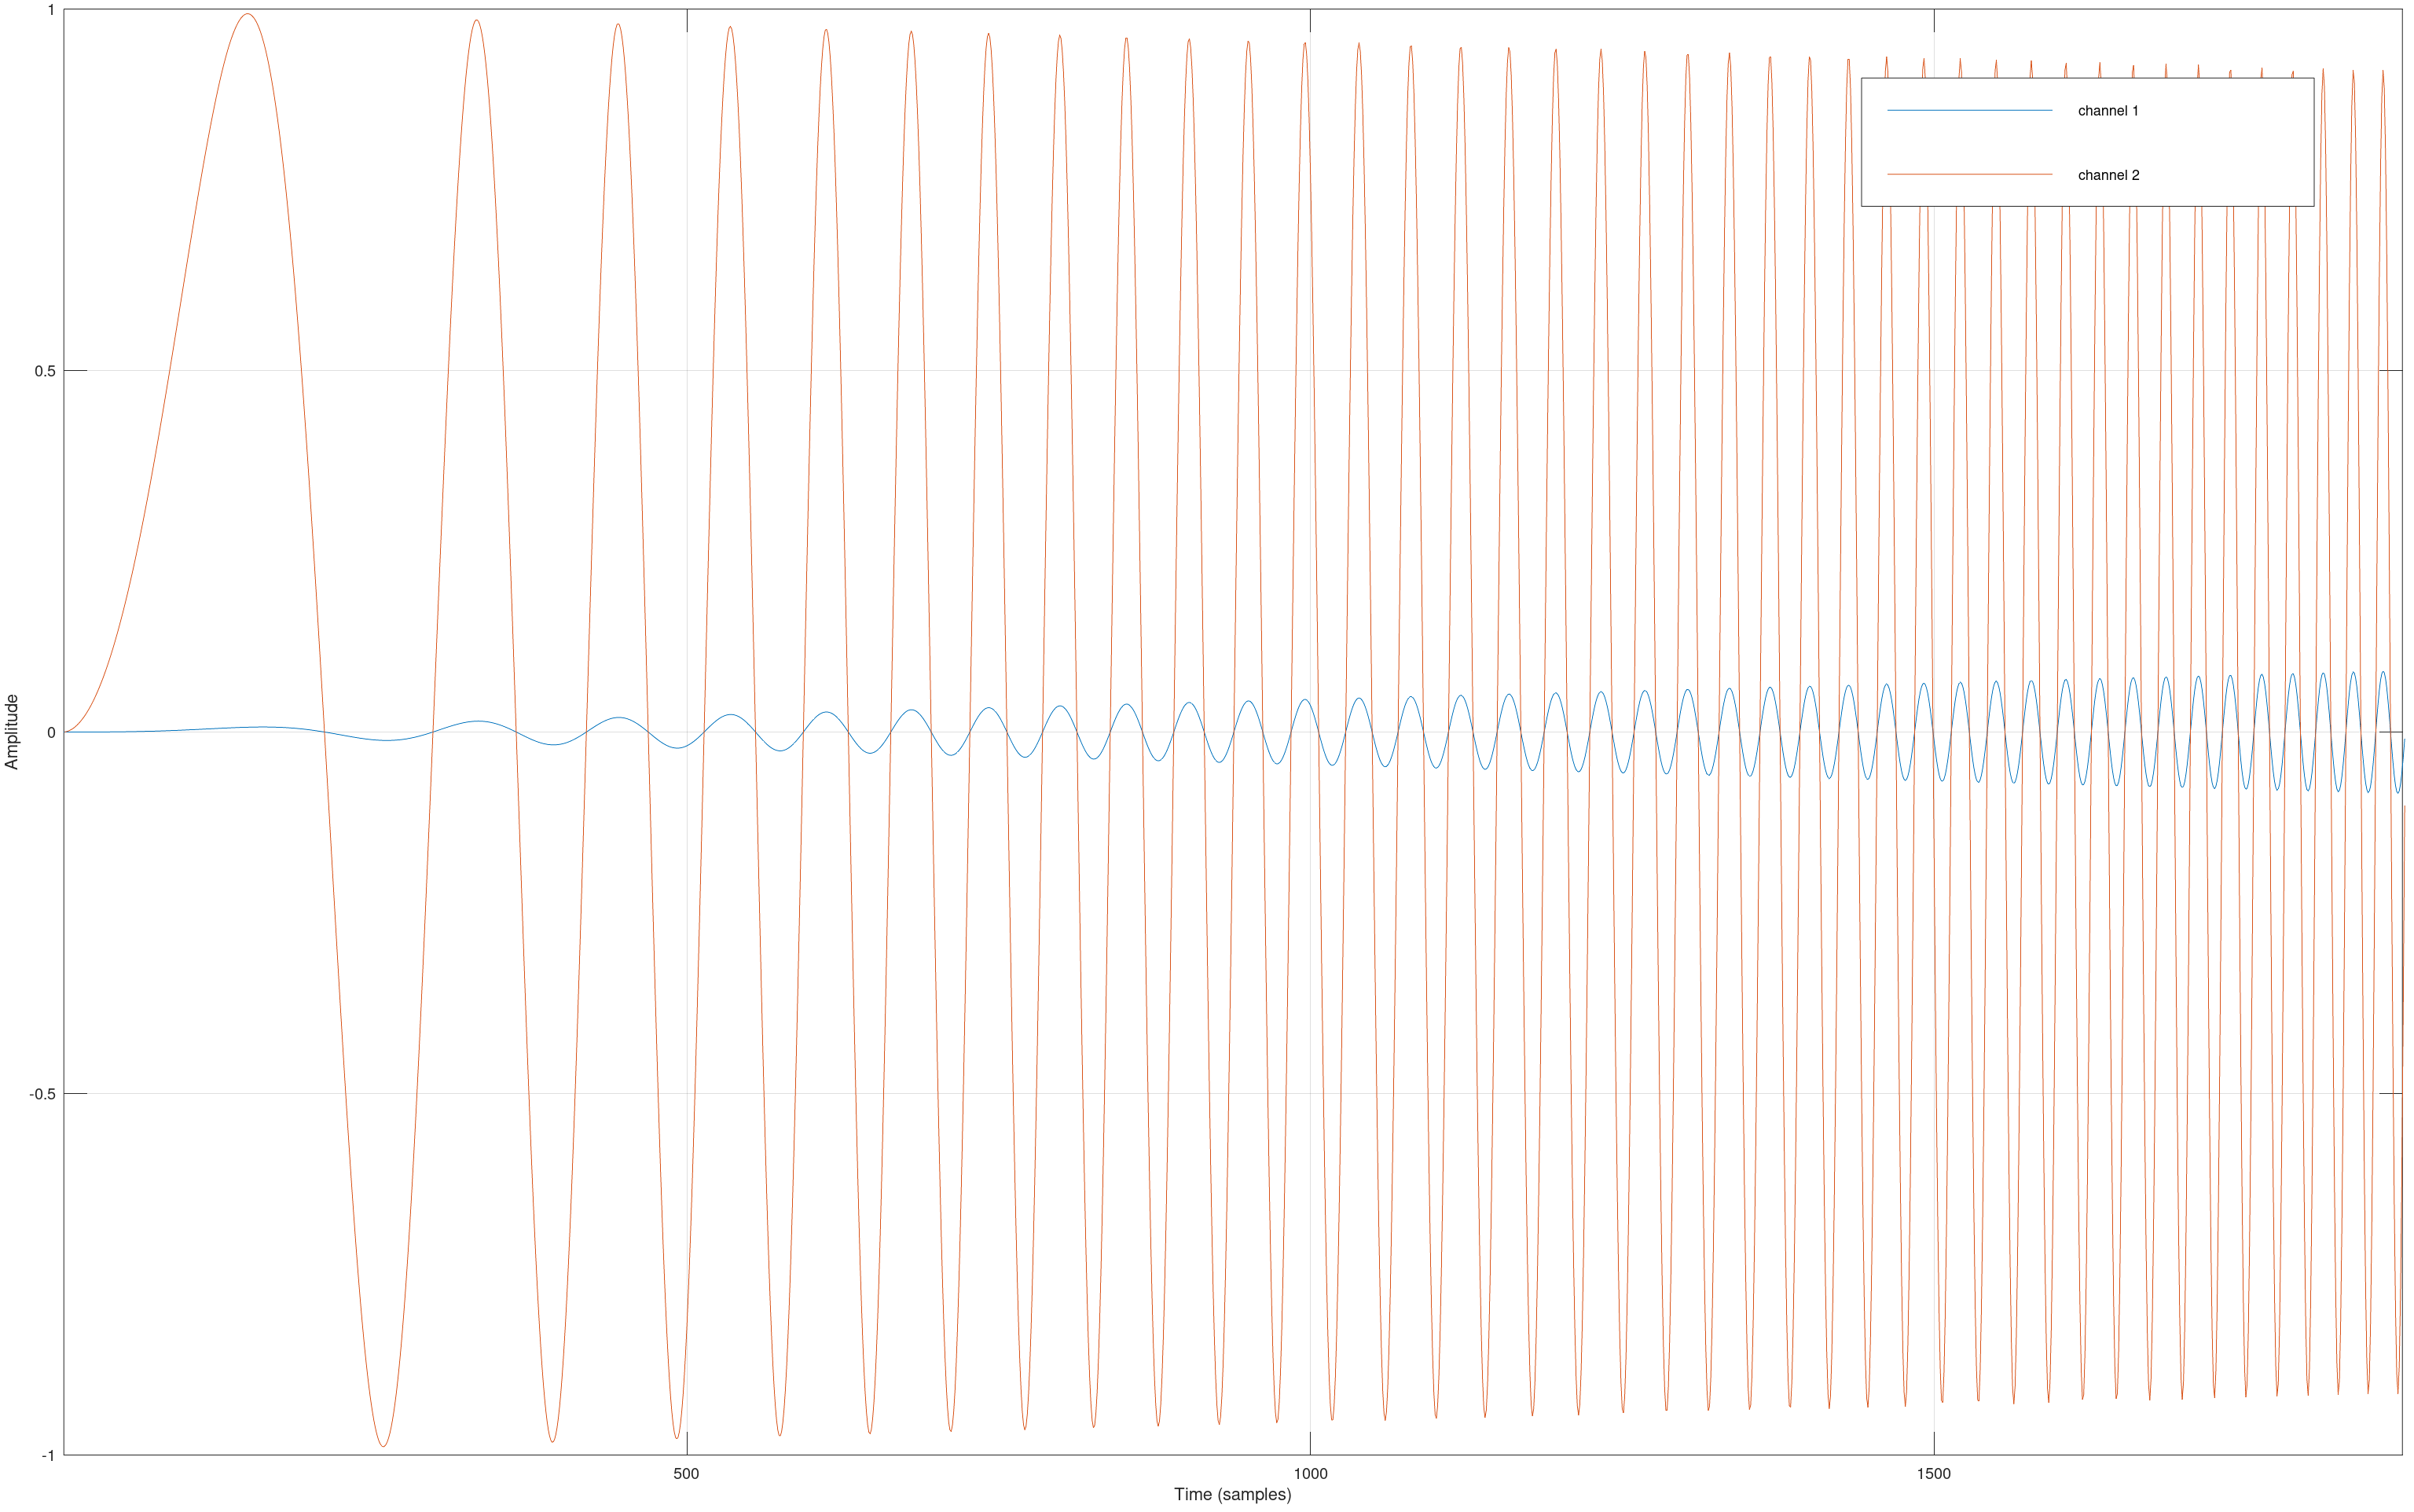
\includegraphics[width=1\columnwidth]{LIN-LR}
\caption{Figure captions should be placed below the figure,
exactly like this.\label{fig:example}}
\end{figure}

%\section{Citations}
%All bibliographical references should be listed at the end, inside a section named ``REFERENCES''. References must be numbered in order of appearance. You should avoid listing references that do not appear in the text.
%
%Reference numbers in the text should appear within square brackets, such as in~\cite{Someone:00} or~\cite{Someone:00,Someone:04,Someone:09}. The reference format is the standard IEEE one. We highly recommend you use BibTeX
%to generate the reference list.
%
%\section{Conclusions}
%Please, submit full-length papers. Submission is fully electronic and automated through the Conference Web Submission System. \underline{Do not} send papers directly by e-mail.
%
%
%\begin{acknowledgments}
%At the end of the Conclusions, acknowledgements to people, projects, funding agencies, etc. can be included after the second-level heading  ``Acknowledgments'' (with no numbering).
%\end{acknowledgments}

%%%%%%%%%%%%%%%%%%%%%%%%%%%%%%%%%%%%%%%%%%%%%%%%%%%%%%%%%%%%%%%%%%%%%%%%%%%%%
%bibliography here
\bibliography{smc2020bib}

\end{document}
